
\documentclass[crop,tikz]{standalone}
\usepackage[utf8]{inputenc}
\usepackage{tikz}
\usepackage{pgfplots}
\pgfplotsset{compat=newest}
\usepgfplotslibrary{groupplots}
\begin{document}

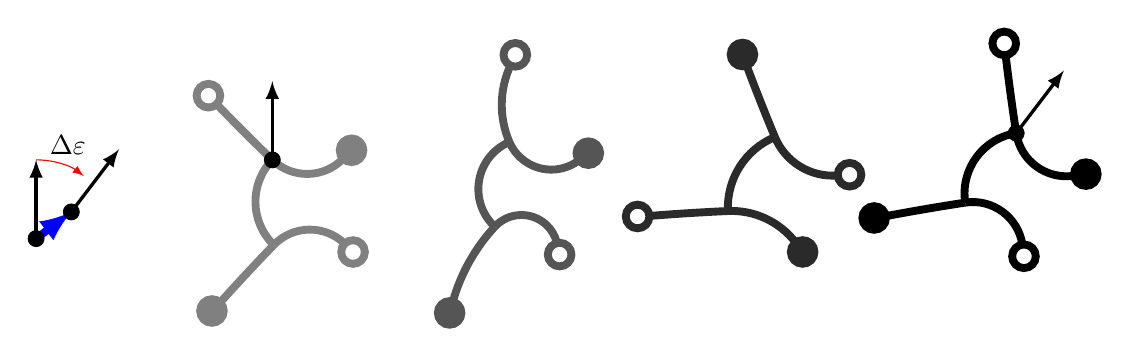
\begin{tikzpicture}[scale=1]%%%% POSE 0
\begin{scope}[xshift=0 cm]

\def\col{black!50.0}
\def\lw{1mm}
\def\alpi{2.000000}
\def\beti{90.000000}
\def\gam{90.000000}
\def\alpii{2.000000}
\def\betii{90.000000}
\def\gamh{45.000000}

\def\eps{90.000006}
\def\ci{44.000006}
\def\cii{135.000006}
\def\ciii{316.000006}
\def\civ{225.000006}

\def\ri{28.647887}
\def\rii{0.636620}
\def\rg{0.763944}
\def\riii{28.647890}
\def\riv{0.636620}

\path (0.000000, -0.000000)coordinate(F1);

\draw[\col, line width=\lw] (F1)arc(180+\ci:180+\ci+\alpi:\ri)coordinate(OM);
\draw[\col, line width=\lw] (OM)arc(180+\ci+\alpi:180+\ci+\alpi+\beti:\rii)coordinate(F2);
\draw[\col, line width=\lw] (OM)arc(90+\ci+\alpi:90+\ci+\alpi+\gam:\rg)coordinate(UM);
\draw[\col, line width=\lw] (UM)arc(\gam+\ci+\alpi:\gam+\ci+\alpi+\alpii:\riii)coordinate(F3);
\draw[\col, line width=\lw] (UM)arc(\gam+\ci+\alpi:\gam+\ci+\alpi-\betii:\riv)coordinate(F4);

\draw[\col, line width=\lw] (F1)++(134.000006 :.15) circle(.15);
\draw[\col, line width=\lw, fill] (F2)++(45.000006 :.15) circle(.15);
\draw[\col, line width=\lw, fill] (F3)++(226.000006 :.15) circle(.15);
\draw[\col, line width=\lw] (F4)++(315.000006 :.15) circle(.15);
\path (OM)coordinate(start); 
\draw[very thick, -latex] (OM)--++(\eps:1); 
\draw[fill] (OM)circle(.1); 
\end{scope} 



%%%% POSE 1
\begin{scope}[xshift=3 cm]

\def\col{black!66.6666666667}
\def\lw{1mm}
\def\alpi{48.000000}
\def\beti{104.000000}
\def\gam{114.000000}
\def\alpii{27.000000}
\def\betii{124.000000}
\def\gamh{57.000000}

\def\eps{80.234841}
\def\ci{335.234841}
\def\cii{127.234841}
\def\ciii{344.234841}
\def\civ{193.234841}

\def\ri{1.193668}
\def\rii{0.579609}
\def\rg{0.650728}
\def\riii{2.334272}
\def\riv{0.462064}

\path (0.730871, 0.490496)coordinate(F1);

\draw[\col, line width=\lw] (F1)arc(180+\ci:180+\ci+\alpi:\ri)coordinate(OM);
\draw[\col, line width=\lw] (OM)arc(180+\ci+\alpi:180+\ci+\alpi+\beti:\rii)coordinate(F2);
\draw[\col, line width=\lw] (OM)arc(90+\ci+\alpi:90+\ci+\alpi+\gam:\rg)coordinate(UM);
\draw[\col, line width=\lw] (UM)arc(\gam+\ci+\alpi:\gam+\ci+\alpi+\alpii:\riii)coordinate(F3);
\draw[\col, line width=\lw] (UM)arc(\gam+\ci+\alpi:\gam+\ci+\alpi-\betii:\riv)coordinate(F4);

\draw[\col, line width=\lw] (F1)++(425.234841 :.15) circle(.15);
\draw[\col, line width=\lw, fill] (F2)++(37.234841 :.15) circle(.15);
\draw[\col, line width=\lw, fill] (F3)++(254.234841 :.15) circle(.15);
\draw[\col, line width=\lw] (F4)++(283.234841 :.15) circle(.15);
\end{scope} 



%%%% POSE 2
\begin{scope}[xshift=6 cm]

\def\col{black!83.3333333333}
\def\lw{1mm}
\def\alpi{2.000000}
\def\beti{72.000000}
\def\gam{70.000000}
\def\alpii{2.000000}
\def\betii{55.000000}
\def\gamh{35.000000}

\def\eps{56.581369}
\def\ci{20.581369}
\def\cii{93.581369}
\def\ciii{272.581369}
\def\civ{216.581369}

\def\ri{27.981490}
\def\rii{0.795770}
\def\rg{0.970139}
\def\riii{28.647759}
\def\riv{1.026389}

\path (0.730871, 0.490496)coordinate(F1);

\draw[\col, line width=\lw] (F1)arc(180+\ci:180+\ci+\alpi:\ri)coordinate(OM);
\draw[\col, line width=\lw] (OM)arc(180+\ci+\alpi:180+\ci+\alpi+\beti:\rii)coordinate(F2);
\draw[\col, line width=\lw] (OM)arc(90+\ci+\alpi:90+\ci+\alpi+\gam:\rg)coordinate(UM);
\draw[\col, line width=\lw] (UM)arc(\gam+\ci+\alpi:\gam+\ci+\alpi+\alpii:\riii)coordinate(F3);
\draw[\col, line width=\lw] (UM)arc(\gam+\ci+\alpi:\gam+\ci+\alpi-\betii:\riv)coordinate(F4);

\draw[\col, line width=\lw, fill] (F1)++(110.581369 :.15) circle(.15);
\draw[\col, line width=\lw] (F2)++(3.581369 :.15) circle(.15);
\draw[\col, line width=\lw] (F3)++(182.581369 :.15) circle(.15);
\draw[\col, line width=\lw, fill] (F4)++(306.581369 :.15) circle(.15);
\end{scope} 



%%%% POSE 3
\begin{scope}[xshift=9 cm]

\def\col{black!100.0}
\def\lw{1mm}
\def\alpi{2.000000}
\def\beti{90.000000}
\def\gam{90.000000}
\def\alpii{2.000000}
\def\betii{90.000000}
\def\gamh{45.000000}

\def\eps{52.713078}
\def\ci{6.713078}
\def\cii{97.713078}
\def\ciii{278.713078}
\def\civ{187.713078}

\def\ri{28.644120}
\def\rii{0.645449}
\def\rg{0.773657}
\def\riii{29.318147}
\def\riv{0.636698}

\path (1.020108, 0.622552)coordinate(F1);

\draw[\col, line width=\lw] (F1)arc(180+\ci:180+\ci+\alpi:\ri)coordinate(OM);
\draw[\col, line width=\lw] (OM)arc(180+\ci+\alpi:180+\ci+\alpi+\beti:\rii)coordinate(F2);
\draw[\col, line width=\lw] (OM)arc(90+\ci+\alpi:90+\ci+\alpi+\gam:\rg)coordinate(UM);
\draw[\col, line width=\lw] (UM)arc(\gam+\ci+\alpi:\gam+\ci+\alpi+\alpii:\riii)coordinate(F3);
\draw[\col, line width=\lw] (UM)arc(\gam+\ci+\alpi:\gam+\ci+\alpi-\betii:\riv)coordinate(F4);

\draw[\col, line width=\lw] (F1)++(96.713078 :.15) circle(.15);
\draw[\col, line width=\lw, fill] (F2)++(7.713078 :.15) circle(.15);
\draw[\col, line width=\lw, fill] (F3)++(188.713078 :.15) circle(.15);
\draw[\col, line width=\lw] (F4)++(277.713078 :.15) circle(.15);
\path (OM)coordinate(end); 
\draw[very thick, -latex] (OM)--++(\eps:1); 
\draw[fill] (OM)circle(.1); 
\end{scope} 



\draw[line width=1mm, latex-, blue] (end)++(-12,-1)coordinate(end_)--($(start)+(-3,-1)$)coordinate(start_) ;
\draw[-latex, red] (start_)++(90:1)arc(90:52.7130781159:1);
\path (start_)++(71.35653905795125:1)node[anchor=251.35653905795124]{$\Delta \varepsilon$};\draw[fill] (start_)circle(.1); 
\draw[very thick, -latex] (start_)--++(90:1); 
\draw[fill] (end_)circle(.1); 
\draw[very thick, -latex] (end_)--++(52.7130781159:1); 
% This file was created by matplotlib2tikz v0.6.18.

\end{tikzpicture}
%% End matplotlib2tikz content %% 
\end{document}